\chapter{Approaches}
In this chapter, we will explain the approaches in this work. Firstly, confronting with the limitations of concrete dropout, we propose another version of concrete dropout, which is called multiple dropout(multi-drop). Secondly, we introduce the modified architecture of ResNet50 in order to make use of techniques introduced in theoretical background chapter.Thirdly, introduce the combination of BNN and CRF in this work, where CRF works as a post-processor to capture the relationship between random variables. Last but not least, the framework for continuous learning with our approaches is introduced in the last section.

\section{Multiple dropout}
From figure \ref{fig:dropout} and expression of approximate distribution in equation \ref{appro_dist_form}, we choose only one probability of Bernoulli distributed random variable for each layer, therefore random vector $\bld p_i = [p_i]^{D_{i-1}}$ for $i$-th layer, which stacks same value into a vector. While the dropout regularization term pushes the probability of Bernoulli to 0.5 to maximize its entropy, the expected likelihood term tries to increase the probability because decreasing probability will lead to a different model with lower capacity and thus low performance. An equilibrium state between them should be achieved in training. With concrete dropout introduced above, we could extend dropout for each hidden units instead of each layer(cf. figure \ref{fig:multi-drop}), which means random vector $\bld p_i = [p_i^k]_{k=1}^{D_{i-1}}$. While the first term in gradients computation stays the same, the second term should be modified to:
\begin{equation} 
\begin{aligned}\label{KL_grad_multi}
\frac{\partial KL(q_{\theta}(\bld \omega)||p(\bld \omega))}{\partial \theta} 
&\approx \frac{\partial \sum_{i=1}^{L}\lambda||\bld M_{i}||^{2}- \beta \mathcal H(\bld p_{i})}{\partial \theta}  \\
&= \frac{\partial}{\partial \theta} \big( \sum_{i=1}^{L}\lambda||\bld M_{i}||^{2}- \beta \sum_{k=1}^{D_{i-1}}(-p_i^k\text{log}p_i^k - (1-p_i^k)\text{log}(1-p_i^k))\big)
\end{aligned}
\end{equation}  

The reasons behind multi-drop are as following:
\begin{itemize}
\item to increase flexibility in tuning variational parameters. The tunability of parameter of Bernoulli random variable in the likelihood term is low because there is only single parameter controlling the entire layer. As is observed in the experiments(cf.figure \ref{fig:cdp_dropout2}), these parameters are always increased for each layer. The reason for this is probably that reducing it would lead to low capacity and thus low likelihood. 

\item the solution space of concrete dropout should be a subset of the solution space of multi-drop if all of them are reachable. Because if it's optimal to assign same probability for each hidden units, this can be recovered in training with multi-drop. Otherwise, other optimal solutions of assigning different probabilities to different hidden units could be considered.

\item last but not least, multi-drop can extend the flexibility and diversity of the dropout approximate distribution family by adding more parameters. Hence the truth posterior can be approximated by the approximate posterior better.
 
\end{itemize}

\begin{figure}[h!]
	\begin{center}
		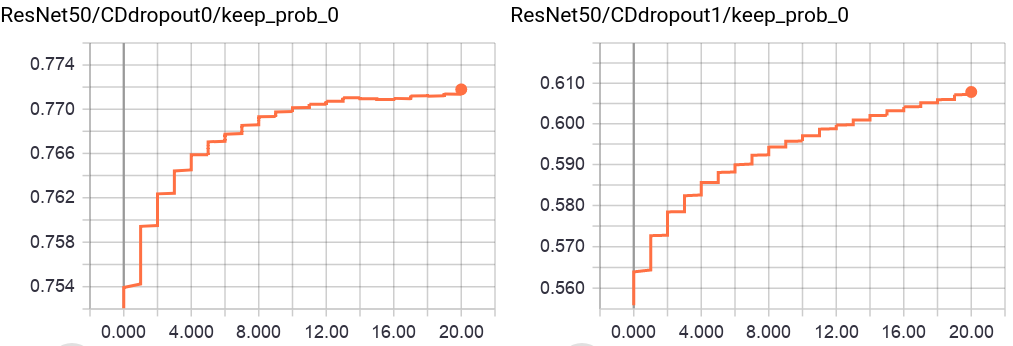
\includegraphics[height=4cm, width=11.5cm]{cdp_dropout1}	
		\label{fig:cdp_dropout1}
	\end{center}
\end{figure}

\begin{figure}[h!]
	\begin{center}
		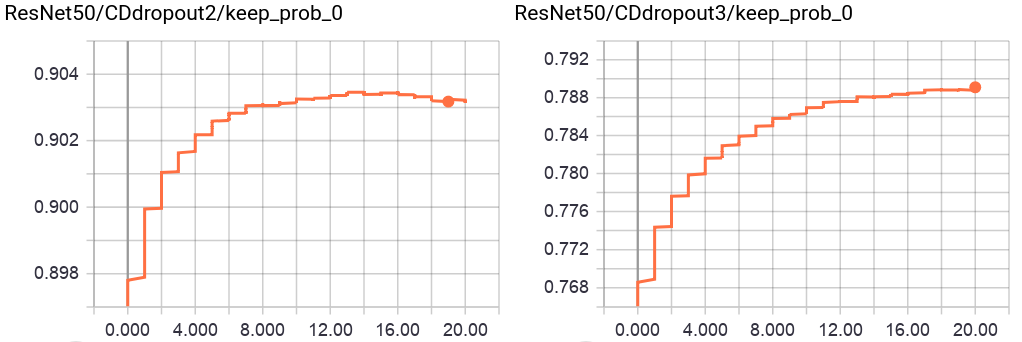
\includegraphics[height=3cm, width=13cm]{cdp_dropout2}	
		\label{fig:cdp_dropout2}
		\caption{Changes along epochs of keep probability in training network with concrete dropout layer.}
	\end{center}
\end{figure}

\begin{figure}[H]
	\begin{center}
		\centering
		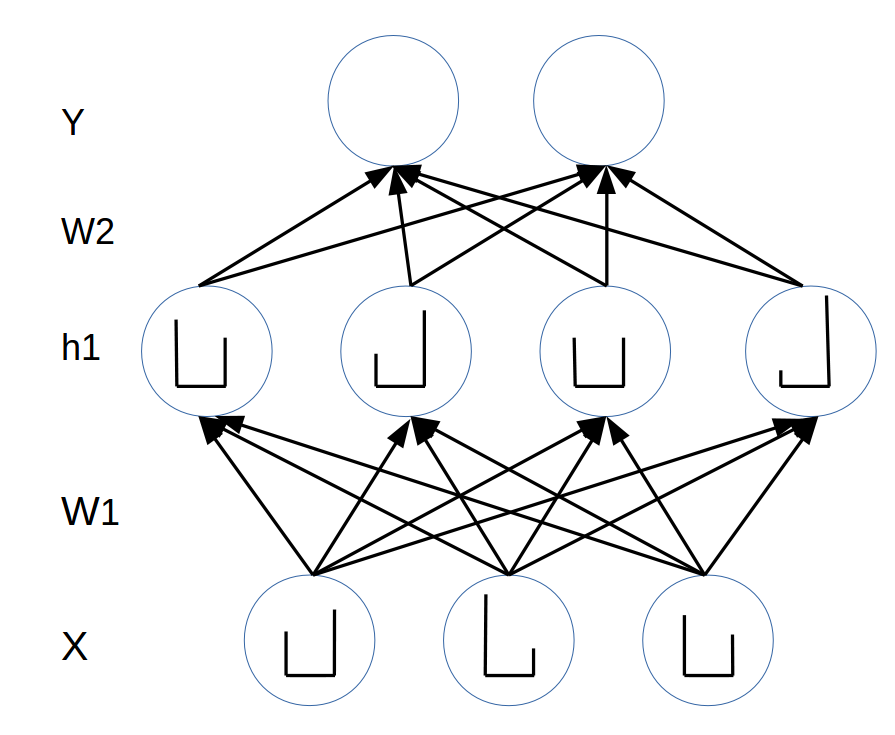
\includegraphics[width=11cm]{multi-drop}
		\caption{Different dropout rates for different hidden units in multi-drop.}		
		\label{fig:multi-drop}
	\end{center}
\end{figure}

\section{Modified network architecture}
After introducing dropout and concrete dropout variational inference, we will describe the modified network architecture in this subsection. The fundamental task in this work is object classification. We choose ResNet50\cite{he2016deep} pre-trained on ImageNet as backbone for fine-tuning because of its strong ability to learn powerful representation for images. However, there is no dropout in original version of ResNet50. If we want to employ dropout variational inference to obtain reliable uncertainty estimation, dropout should be inserted into the network. In this work, we add three fully connected layer with 1024 hidden units , which are initialized from scratch, before the output layer whose dimension needs to be set to the number of classes. Then we add concrete dropout at flatten layer, and these three new added fully connected layer, respectively.
There are three reasons why we modify the network in this way:
\begin{itemize}
	\item Inserting dropout in layers initialized with pre-trained weights will destroy pre-trained features. Because we initialize major part of network with pre-trained weights, hence it would lead to significant drop of performance after fine-tuning if we insert dropout into them. 
	\item According to the suggestions from \cite{srivastava2014dropout}, insertion of dropout reduces the capacity of the model and thus a model with	dropout should have larger capacity than one without dropout. Therefore we add three more fully connected layers to make sure that our model possesses large enough model capacity.
	\item As we have introduced in previous sub-sections, weights are major part of variational parameters. Therefore to have more weights can enhance the flexibility and capacity of approximate distribution family, which improves the quality of approximation.  
\end{itemize}

From figure \ref{fig:modified_net}, we can see the sketch of our modified network architecture. More concretely, we can interpret major parts of network, which do not have dropout inserted, as a deterministic feature extractor. On the other hand, for layers with dropout inserted work as a probabilistic classifier based on aforementioned Bayesian interpretation of dropout. In training, these two parts are trained jointly in order to achieve a better balance and more optimal results. In testing, we need to marginalize possible parameters according to posterior distribution. Layers with dropout should be sampled and run multiple times to produce a predictive distribution of output class.
\begin{figure}[H]
	\begin{center}
		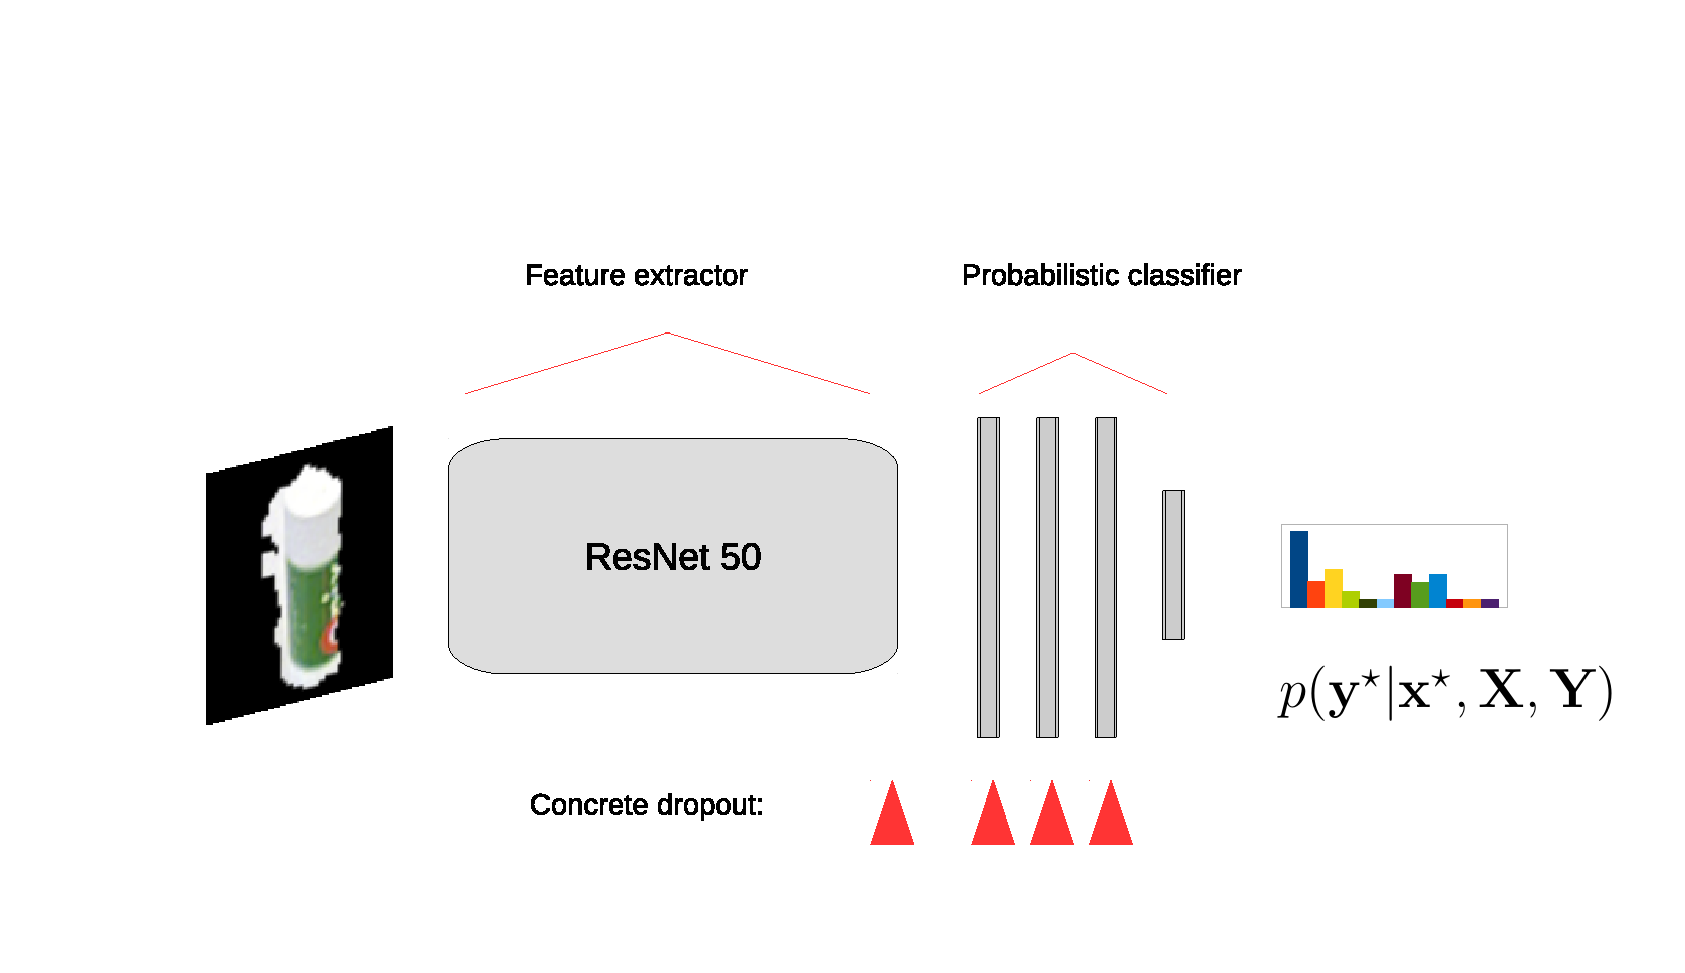
\includegraphics[height=8.5cm, width=15.5cm]{network}
		\caption{Modified network architecture of ResNet50.}		
		\label{fig:modified_net}
	\end{center}
\end{figure}

\section{Combination with CRF}
CRF as a post-processor.
\begin{figure}[H]
	\begin{center}
		\includegraphics[height=9cm, width=15.5cm]{combined_crf}
		\caption{Combination of BNN and CRF.}		
		\label{fig:combined_crf}
	\end{center}
\end{figure}
\section{Proposed approach for continuous learning}

\begin{figure}[H]
	\begin{center}
		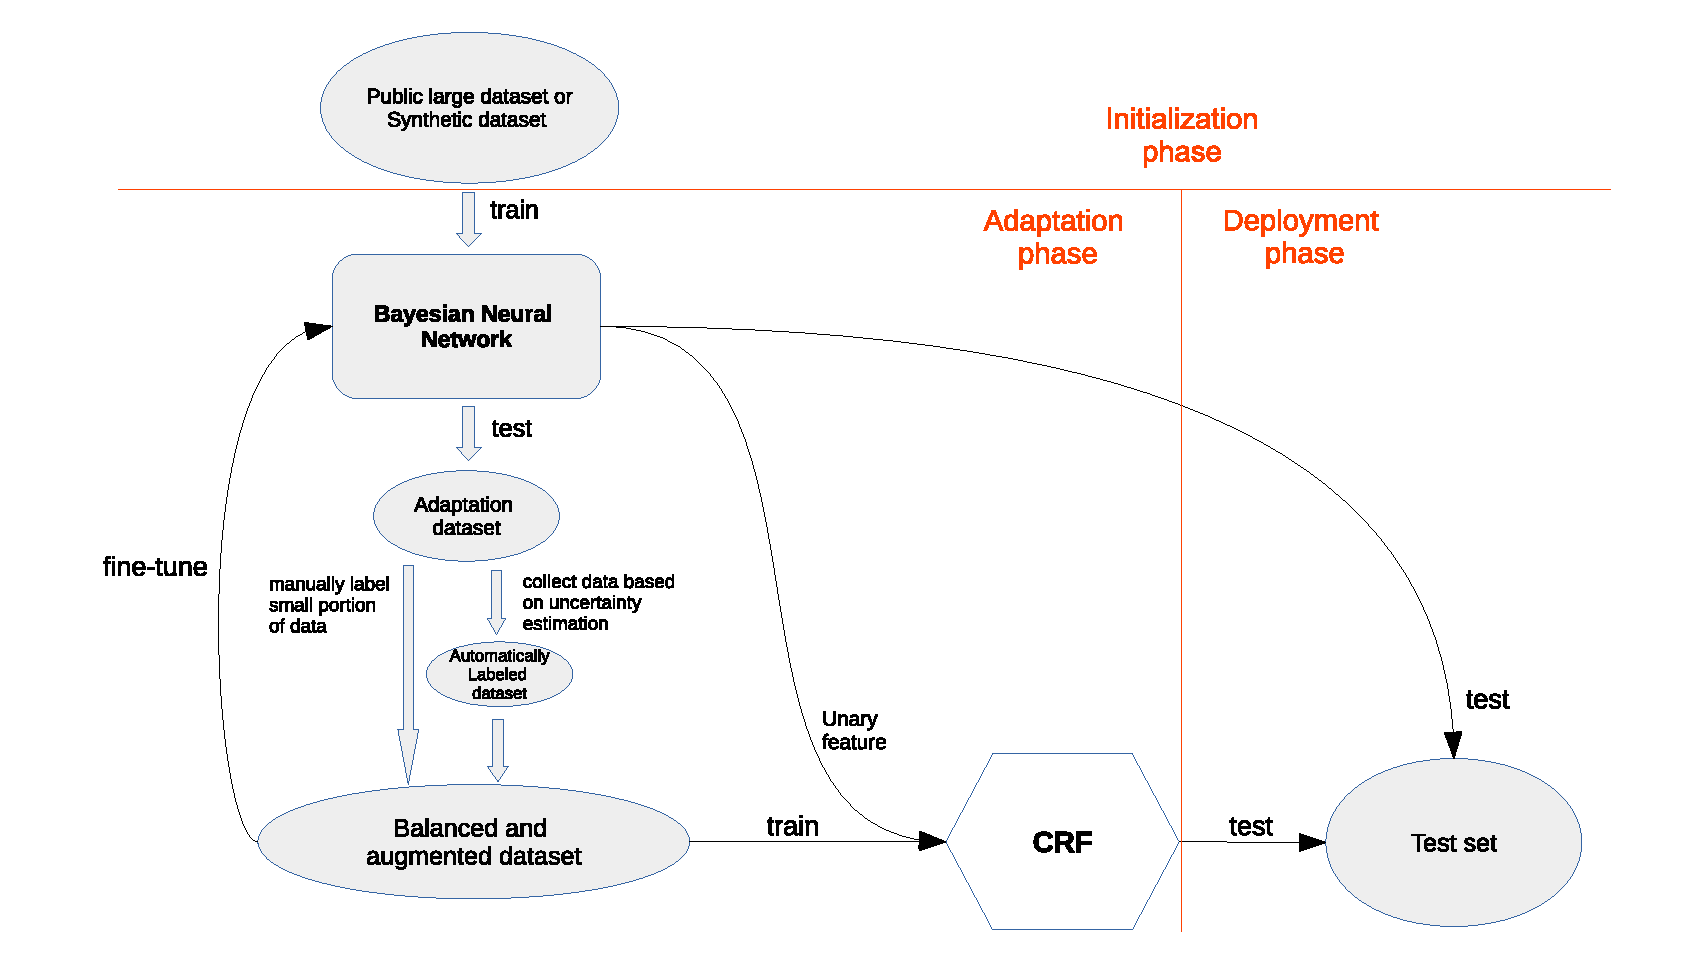
\includegraphics[height=10cm, width=16cm]{con_learn}
		\caption{Approach for continuous learning.}		
		\label{fig:con_learn}
	\end{center}
\end{figure}
